\chapter{\IfLanguageName{dutch}{Literatuurstudie}{Literatuurstudie}}
\label{ch:literatuurstudie}

% Tip: Begin elk hoofdstuk met een paragraaf inleiding die beschrijft hoe
% dit hoofdstuk past binnen het geheel van de bachelorproef. Geef in het
% bijzonder aan wat de link is met het vorige en volgende hoofdstuk.

% Pas na deze inleidende paragraaf komt de eerste sectiehoofding.

Voor we het onderzoek kunnen voeren naar hoe we een impressie kunnen bekomen van een menselijke conversatie-ervaring met behulp van combinaties van narrow ai-technologieen, is het belangrijk om verschillende zaken toe te lichten in deze literatuurstudie die aan bod zullen komen tijdens het onderzoek.

Eerst zal men de geschiedenis van AI even schetsen, om een beeld te kunnen scheppen hoe snel de groei in het domein verloopt.

\section{Waar staat AI vandaag, en hoe snel gaat de evolutie?}
De term 'AI' is een term die we in het huidige tijdperk niet meer kunnen wegdenken. Het is alom bekend en wordt in veel (grote) bedrijven gebruikt voor allerhande toepassingen. Maar hoe zijn we hier geraakt? En is deze evolutie verlopen zoals we pakweg 20 jaar geleden zouden verwacht hebben?

\subsection{De populariteit van AI}
Volgens \cite{brynjolfsson2017artificial} dat zich vooral focust op AI in de bedrijfswereld is AI de dag van vandaag al enorm aanwezig in verschillende bedrijven. Dit komt omdat er voortdurend 'general purpose' technologieën opduiken, dit zijn technologieën die de mogelijkheid hebben om een hele economie te kunnen beïnvloeden en het potentieel hebben om samenlevingen drastisch te veranderen door hun impact op al bestaande sociale en economische structuren. Neem nu bijvoorbeeld de verbrandingsmotor die er voor zorgde dat auto's, truck's,... gecommercialiseerd konden worden door bijvoorbeeld bedrijven zoals UPS of Uber. De meest belangrijke 'general purpose' technologie van deze tijd is machine learning: dit is het vermogen van een machine om te kunnen blijven evolueren en het voortdurend verbeteren van zijn prestaties zonder dat mensen exact moeten uitleggen hoe ze een bepaalde taak moeten volbrengen die hen gegeven wordt. 

Dit is dan ook deels de grootste factor waarom AI de dag van vandaag zo populair is, omdat er economisch, en dus binnen de bedrijfswereld ook enorm veel vooruitgang kan geboekt worden. Zeker de afgelopen jaren is er enorme vooruitgang geboekt om machines taken autonoom te laten uitvoeren.

\subsection{Wat kan AI momenteel al?}

AI, of Artificiële intelligentie wordt meestal gezien als de capaciteit van machines om menselijke taken uit te voeren, voornamelijk zaken die te maken hebben met congnitieve functies zoals luisteren, kijken, spreken,... 

Volgens enquetes van \cite{benbya2020artificial} wordt er gesuggereerd dat minder dan de helft van de organisaties zinvolle AI projecten hebben lopen, of het vooruitzicht hebben dat deze zullen plaatsvinden, dus hier is nog veel ruimte voor groei. 

Maar wat is het dan juist? Waar is AI nuttig voor, en waarvoor wordt het gebruikt? Dit zal hier verder besproken worden.

\subsubsection{Business}
Ook al blijven de meeste grote AI-projecten die opgezet worden in de bedrijfswereld experimenteel, of een proof of concept, is het niet zo dat er geen enkel bedrijf is waar AI gebruikt wordt. 

Toch wordt AI effectief gebruikt en kan men uit een enquete, afgenomen door Deloitte, waar bedrijfsleiders werden gevraagd waarvoor ze AI gebruiken, het onderstaande afleiden (percentages betekenen hoe vaak de antwoorden zijn voorgekomen bv. 'om keuzes maken te vergemakkelijken' kwam voor in 1 op 4 van de enquetes, er konden tevens ook meerdere antwoorden worden geselecteerd)

\begin{itemize}
    \item 28\% om processen te vergemakkelijken
    \item 25\% om bestaande producten of services te verbeteren
    \item 23\% om nieuwe producten of services te creëren
    \item 21\% om keuzes maken te vergemakkelijken
    \item 20\% om kosten te verlagen
\end{itemize}

Een interessant gegeven is dat AI vaak genoemd wordt om het aantal werknemers te verminderen in een bedrijf, toch werd dit maar in 11\% van de enquetes genoemd. 

Echter in deze tendens wordt er nu een verschuiving gemerkt. Waar werkgevers initieel enkel focuste op het gebruiken van AI om bepaalde specifieke workflows, processen en repetitief werk te automatiseren, wordt er nu meer gekeken om AI in te zetten voor niet systematische congitieve taken, die zelfs keuzes kunnen maken en problemen kunnen oplossen. Zelfs creativiteit is iets waarvoor AI momenteel kan gebruikt worden. Dit is iets wat pakweg 5 jaar geleden buiten de technische scope van AI viel. 

Eerst is het belangrijk om een goed beeld te vormen van wat er momenteel (technologisch) mogelijk is met AI.

\subsubsection{Technologie}
Het is belangrijk om een beeld te scheppen van de evolutie van de technologie achter AI tot dusver.

Eerst is het belangrijk om te benadrukken dat de term 'AI' redelijk breed is.

Uit de studie van \cite{benbya2020artificial} kan men AI types bekijken van uit 3 inzichten:
\begin{itemize}
    \item Gebaseerd op functie
    \item Gebaseerd op technologie
    \item Gebaseerd op intelligentie
\end{itemize}

We kunnen deze 3 brede takken nog iets beter toelichten per tak.

\subsubsection{Gebaseerd op functie}

    Hier wordt het onderscheid gemaakt tussen vier soorten artificiële intelligentie. Namelijk conversationale, biometrische, algoritmische en robotische AI. Hier gaat het dus louter om de functie waarvoor de AI gebruikt wordt. 
    
    Zo is conversationele AI sinds de opkomst van OpenAI en ChatGPT zeer populair, dit is zoals het woord het wel al doet vermoeden, een ai die in staat is om menselijke taal te herkennen, en te begrijpen. Dit doormiddel van tekst -en stemherkenning. Conversationele AI heeft bijgevolg het meeste kans om meer complexe taken te kunnen uitvoeren, omdat het duidelijker kan gemaakt worden wat de opdracht is, als de AI het taalmodel begrijpt van de opdrachtgever.
    
    Biometrische AI gaat dan weer om met het fysiologische aspect van de mens en heeft als functie bijvoorbeeld vingerafdrukken herkennen, iris scanner,... maar ook bijvoorbeeld het herkennen van gedragskenmerken zoals een handtekening, stem,... 
    
    Algoritmische AI heeft voornamelijk te maken met machine learning (ML) algoritmen. Dit zijn een aantal instructies die een computer kan uitvoeren. Dit kan bijvoorbeeld zijn om een bepaalde specifieke taak aan te leren aan de AI.

    Robotische AI slaat op fysieke robots, deze worden al geringe tijd gebruikt in bijvoorbeeld fabrieken. Robots met AI kunnen hun omgeving waarnemen, begrijpen, leren en hier acties op ondernemen. Dit draagt bij aan het feit dat robots een groot aantal taken kunnen uitvoeren, dit kan gaan over mensen assistentie bieden bij een aantal taken, of het identificeren van objecten, en op basis van deze objecten bepaalde taken uitvoeren.

\subsubsection{Gebaseerd op technologie}

    Hier is het onderscheid gebaseerd op de technologie die gebruikt wordt in het AI systeem. Dit gaat vooral over machine learning, deep learning, neural networks, natural language processing, rule-based expert systemen, robotic process automation en robots.
    
    Machine learning kan men opzich nog eens opdelen in 3 takken, namelijk reinforcement learning, supervised learning en unsupervised learning.
    Kort uitgelegd: Reinforced learning slaat op een AI dat kan leren uit ervaring, zonder menselijke invloed. Supervised learning is wanneer een AI leert van een dataset waarmee het getrained wordt. Unsupervised learning is wanneer een AI patronen kan herkennen in data dat niet gelabeled is, en waarvan het resultaat nog niet gekend is.
    
    Deep learning is een klasse van machine learning waarbij de AI kan leren zonder supervisie van een persoon. Het kan zichzelf trainen via zowel gelabelde als ongelabelde data. Een welgekend voorbeeld hier van is spraak -en afbeeldingsherkenning.
    
    Neural networks zijn algoritmes die proberen onderliggende relaties uit een dataset te halen via een proces dat de werking van het menselijk brein probeert na te bootsen.
    
    Natural language processing kwam daarnet al aan bod en slaat op het feit dat een AI de mogelijkheid heeft om een taal te herkennen en te begrijpen. bv. ChatGPT
    
    Rule based expert systems zijn systemen waarbij er een aantal gepredefineerde regels worden opgesteld door een persoon. Deze worden dan gevolgd door deze AI, vandaar de naam Rule based.
    
    Robotic process automation systemen zijn systemen die gebouwd zijn om bepaalde digitale taken te automatiseren, dit kan bijvoorbeeld het inwisselen van een credit kaart zijn, waar er een aantal vaste processen dienen uitgevoerd worden, deze gebeuren dan via de AI.
    
    Robots kwamen daarnet ook al aan bod, en slaat op het automatisch bedienen van machines. Bijvoorbeeld in een fabriek.
    
    \newpage
    
\subsubsection{Gebaseerd op intelligentie}

    Dit slaat op de intelligentie van de AI. En dit kan men opdelen in 3 delen.
    \begin{itemize}
        \item Artificial Narrow Intelligence
        \item Artificial General Intelligence
        \item Artificial Super Intelligence
    \end{itemize}

    Artificial Narrow Intelligence (ANI) en Artificial General Intelligence (AGI) worden verder in deze literatuurstudie besproken, dus hier zal men momenteel niet te diep op in gaan. 
    
    Artificial Narrow Intelligence slaat op een AI dat vaak maar de mogelijkheid heeft om één bepaald probleem op te lossen. En niet in staat is om vaardigheden die het kent om dit bepaald probleem op te lossen, over te dragen naar een ander domein. 
    
    Artificial General Intelligence slaat op een AI die streeft naar het leren van zaken op menselijk niveau. Het kan vaardigheden van het ene domein naar het andere domein overdragen en kan ook linken leggen tussen bepaalde oplossingen voor gegeven problemen. Het kan leren zoals een mens dit kan. Dit zal op vlak van kennis dus de impressie zijn die men wilt geven in het geval van onze case.
    
    Artificial Super Intelligence is een theoretische vorm van een AI, waar het mogelijk zou zijn om de mensenlijke aspecten te overstijgen. De theorie zegt dat wanneer men er in slaagt om een AGI te ontwikkelen dat deze general intelligence zonder problemen slimmer en beter zal blijven worden en uiteindelijk meer capaciteiten kan ontwikkelen dan de mens en zo vervolgens zal evolueren tot een super intelligence. 


\subsection{Recente veranderingen in het domein}

Om de evolutie verder te schetsen, is het interessant om de laatste evoluties binnen het domein even te schetsen, die ook deels de reden zijn waarom deze bachelorproef plaats vind binnen dit domein. 

\subsubsection{ChatGPT}
ChatGPT is een openbare website die ontwikkeld is door OpenAI.

OpenAI is een bedrijf gevestigd in de Verenigde Staten dat zich richt op onderzoek en ontwikkeling op het gebied van kunstmatige intelligentie. Het bedrijf heeft als doel om uiteindelijk kunstmatige algemene intelligentie te creëren. Zo zijn ze momenteel pionier in de GPT3, GPT3.5 en ondertussen GPT4 technologie, hier over later meer. Ook zijn zij de ontwikkelaars van DALL-E 2, een AI software die gebruik maakt van GPT om realistische afbeeldingen en kunst te genereren aan de hand van natuurlijke taal. Ten slotte zijn ze ook het bedrijf achter ChatGPT, een zeer bekend product die als maar toeneemt in populariteit.

Zoals waarschijnlijk wel al duidelijk was uit de vorige alinea is ChatGPT dus een AI gebaseerd op het GPT taalmodel. ChatGPT zelf gedraagt zich eigenlijk zoals een chatbot waar je zo goed als alles aan kan vragen.

ChatGPT is dus een zeer geavanceerde chatbot die in staat is om een groot aantal tekstgebaseerde verzoeken af te handelen, waaronder het beantwoorden van eenvoudige vragen en het uitvoeren van meer geavanceerde taken zoals het genereren van marketingberichten en het begeleiden van individuen bij lastige discussies over productiviteitsproblemen, en zelfs bugs uit code halen is niet onmogelijk. ChatGPT kan dit doen door gebruik te maken van zijn uitgebreide databank en GPT technologie om gebruikersverzoeken te begrijpen en te interpreteren en vervolgens passende antwoorden te genereren in bijna natuurlijke mensenlijke taal. 

Er zijn bepaalde bedrijfs sectoren waar een AI dat enorm goed is in taalverwerking een enorme evolutie kan betekenen. Zo kan het de ideale tool zijn voor het afhandelen van eenvoudige klantenservicevragen, zoals de chat functie op websites. De mogelijkheid om grote hoeveelheden tekst te analyseren en interpreteren kan ook waardevol zijn in de juridische sector, waarbij het mogelijk kan helpen bij onderzoeks- en documentvoorbereidingstaken. Daarnaast kan de mogelijkheid van ChatGPT om toezicht te houden op de kwaliteit van geschreven werk nuttig zijn in het onderwijsveld, waarbij het mogelijk kan helpen bij het beoordelen en feedback geven op studentenopdrachten.

Naast zijn praktische toepassingen maakt de mogelijkheid van ChatGPT om mensachtige taal te genereren en complexe taken uit te voeren, het dus een belangrijke innovatie in het veld van natuurlijke taalverwerking en kunstmatige intelligentie.

\cite{lund2023chatting}

\newpage

\section{Artificial Narrow Intelligence}

Wat veel mensen niet weten is dat wanneer men refereert naar AI of Artificial Intelligence, is dat men eigenlijk praat over Artificial Narrow Intelligence, waarover in deze sectie heel wat informatie zal gegeven worden. Omdat men tijdens het onderzoek op zoek zal gaan naar combinaties van verschillende Narrow AI's.

De grootste groei van AI de afgelopen jaren kan men vinden in enerzijds perceptie en anderzijds cognitie. In perceptie is de grootste evolutie gebeurd op vlak van spraakherkenning. Dit is iets dat door tal van mensen wordt gebruikt, denk bijvoorbeeld maar aan Alexa, Siri,... Hetzelfde geldt voor afbeeldingsherkenning.

Wetende dat bijvoorbeeld spraakherkenning pas sinds de zomer van 2016 enorm is beginnen groeien kan men wel stellen dat evolutie in AI enorm snel kan gaan.

 \autocite{brynjolfsson2017artificial}

\subsection{Technische aspecten}

Als we gaan kijken naar wat Artifical Narrow Intelligence juist technisch inhoudt, kan men stellen dat dit een AI is die gebouwd is om een bepaalde taak uit te voeren binnen een bepaald domein. Eventuele kennis die deze AI vergaart door deze taak uit te voeren zal niet automatisch worden gebruikt om andere taken uit te voeren buiten dit domein. 

Wanneer we ons iets meer gaan toespitsen op AI binnen bedrijven, dan merkt men nog steeds dat het gaat om narrow AI’s. Deze worden gebruikt om bepaalde cognitieve (mensenlijke) taken uit te voeren en te automatiseren. Dit zijn vaak fysieke processen zoals het bewegen van objecten, voelen, waarnemen, problem solving, keuzes maken en innoveren. 

Bij de meeste organisaties is het gebruiken van AI binnen het bedrijf nog steeds experimenteel. En dit komt deels door de beperking van een Narrow Artificial Intelligence dat zich vaak enkel toespitst op een enkele taak.

Narrow Artificial Intelligence is dus nog steeds maar in staat om één specifiek probleem op te lossen en niet in staat vaardigheden van het ene domein naar het andere over te dragen. Echter nog niet zo lang geleden beginnen AI-programma’s zoals bijvoorbeeld de GPT-3, GPT-3.5 en GPT-4 taalvoorspelling enkele aspecten van algemene intelligentie te vertonen, door verschillende narrow ai's te combineren, zoals in een voorgaande sectie besproken werd.

\autocite{benbya2020artificial}

\newpage

\section{Artificial General Intelligence}

In tegenstelling tot Artificial Narrow Intelligence verwijst Artificial General Intelligence naar een AI die op vlak van kennis kan blijven groeien. Hiermee wordt bedoeld dat die verschillende soorten taken, uit verschillende domeinen kan uitvoeren. Door het uitvoeren van deze taken leert de AI bij zoals een mens dit doet en kan hij bijleren om vervolgens taken uit andere domeinen ook te kunnen oplossen. 

Artificial General Intelligence heeft het vermogen om kennis te verwerven en toe te passen, en om te redeneren en te denken, op verschillende gebieden. Je kan stellen dat Artificial General Intelligence streeft naar 'Algemene Intelligentie', zoals dit ook uit de engelse term afgeleid kan worden. 

\subsection{Technische aspecten}

Uit een studie is gebleken dat wanneer we menselijke algemene intelligentie willen toepassen op een AI, die het volgende moet bevatten: \linebreak

\begin{itemize}
    \item Het vermogen om algemene problemen op een niet-domeingebonden manier op te lossen
    \item Het vermogen om specifieke (taakgebonden) en algemene intelligentie samen te gebruiken
    \item Het vermogen om te leren van zijn omgeving, andere ai's en leraren, al dan niet menselijk
    \item Het vermogen om beter te worden in het oplossen van nieuwe soorten problemen naarmate de ai meer ervaring op doet met dit type problemen
\end{itemize}

Het belangrijkste om te onthouden is dat een belangrijk aspect van Artificial General Intelligence draait om het feit dat een systeem autonoom kan leren, en kennis die het verstrekt heeft door een taak te voltooien kan gebruiken om een andere taak op te lossen, ongeacht welk domein deze taak zich in bevindt. 

Het systeem moet kunnen interageren met zijn omgeving en met andere entiteiten in zijn omgeving, dit kunnen ai's of menselijke interacties zijn. De AI leert bij uit deze interacties. Verder is het in staat om verder te bouwen op eerdere ervaringen en de vaardigheden die daar geleerd zijn te onthouden en toe te passen op complexere taken, om zo ook deze af te ronden. Op deze manier leert een Artificial General Intelligence als maar bij en kan het steeds complexere doelen bereiken.

\cite{goertzel2007artificial}

Momenteel komen de huidige AI systemen nog niet volledig in de buurt van de bovenstaande aspecten. Echter is het wel zo dat er in bepaalde gebieden aanwijzingen zijn die duiden op vooruitgang. Een goed voorbeeld daarvan zijn neurale netwerken, deze vormen de basis van een hele boel recente successen in de AI-wereld. Maar ook zij hebben het nog moeilijk om over te schakelen van een taak uit een specifiek domein naar een taak uit een ander domein. Zo is het gemakkelijk om een specifiek geval van een probleem te nemen en zich te richten op het verbeteren van deze prestaties in plaats van te proberen om systemen te bouwen met echt diverse vaardigheden. Zo kan men pas enkel AGI bereiken wanneer het systeem effectief uit zichzelf kan leren uit enkele voorbeelden over een enorm spectrum van domeinen.

\cite{shevlin2019limits}

\newpage

\subsection{Menselijke aspecten}

In deze bachelorproef zal er niet onderzocht worden of men technisch een AGI kan opzetten, dit is met de technologie van vandaag nog niet mogelijk. Echter is het wel zo dat men de menselijke aspecten van een AGI zoals hierboven benoemd is op vlak van kennis, kan in kaart brengen, en kan proberen om te schetsen wanneer men de impressie heeft dat men contact heeft met een AI die menselijk lijkt. 

Hieromtrent is er reeds een zeer bekende  studie rond gebeurd, namelijk de test genaamd de Turing test, door Alan Turing.

\section{Alan Turing-Test}

De Alan Turing-test is een experiment dat in 1950 werd voorgesteld door de Britse wiskundige Alan Turing om te bepalen of een machine in staat is tot menselijk denken. Het idee achter de test is om een machine en een persoon te laten communiceren via een scherm en toetsenbord, zonder dat de desbetreffende persoon weet of hij met een machine of een andere mens praat. Als de machine erin slaagt om de persoon te overtuigen dat het een andere mens is, wordt de machine beschouwd als intelligent. De Turing-test wordt nog steeds gebruikt voor het evalueren van de mensachtige eigenschappen van computers en robots.

\subsection{Verloop test}

In de paper van \cite{warwick2016can} wordt teruggeblikt op een aantal turing testen die door de Royal Society zijn uitgevoerd.

Eerst en vooral is het belangrijk om te weten wat de criteria zijn om te kunnen zeggen dat een AI slaagt voor de Alan Turing test. 

Dit is kort beschreven hoe een test er uit ziet: 

\begin{figure}[htbp]
    \centering
    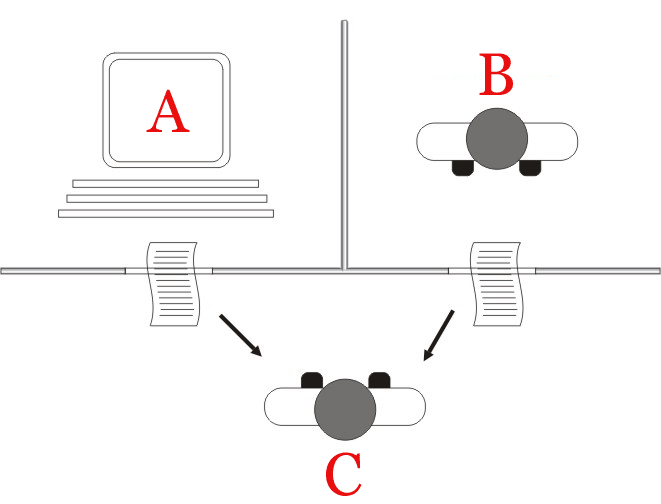
\includegraphics[width=0.5\textwidth]{Turing_test_diagram.png}
    \caption{\cite{Margallo2017}}
    \label{fig:turing test diagram}
\end{figure}

De test bestaat meestal uit enkele personen die vragen zullen stellen aan verschillende tegenpartijen, via een scherm en toetsenbord. Deze tegenpartijen zijn zowel mensen of een machine die er op getraind is om zijn tegenpartij te doen geloven dat het een persoon is. 

Op de ingesteldheid van deze machine is wel al commentaar gekomen omdat er niet bewezen wordt dat de machine ook echt slim is, maar wel dat het de tegenpartij kan misleiden om dit te doen geloven. Daarom wordt de Alan Turing test vaak ook de imitatietest genoemd, omdat de machine een echte persoon imiteert. Echter is dit voor deze bachelorproef nog steeds interessant omdat één van de aspecten die men zal onderzoeken ook te maken heeft met conversaties en het al dan niet herkennen of we met een machine of persoon in contact staat. 

Tijdens deze test krijgt de persoon die probeert te weten of hij een tekstuele conversatie heeft met een mens of robot ongeveer vijf minuten de tijd om vragen te stellen aan zijn tegenpartij. Dit kan dus een mens of een robot zijn. 

Dit herhaalt zich een aantal keer, waar de ondervrager wisselt tussen verschillende tegenpartijen. Na dat deze verschillende gesprekken afgerond zijn dient de ondervrager aan te duiden voor elke entiteit waarmee hij een conversatie heeft gehad of het een robot of mens was.

Om te weten of een machine slaagt voor de Alan Turing test dient de machine, in meer dan 30\% van de testen waarin hij deelgenomen heeft, geïdentificeerd worden als mens. 

Deze bachelorproef zal geen uitbreiding zijn op deze test, aangezien de test zich voornamelijk focust op het conversationele vlak én het effectief laten converseren van een machine met een persoon. In deze bachelorproef zal men meer op zoek gaan naar de grens wanneer men interactie met een AI kan herkennen. En welke artificial narrow ai's men dient te combineren om een gevoel te creeëren dat men met een echt persoon in contact staat, met voornamelijk focus op de menselijke aspecten.

\newpage

\section{Specifieke artificial narrow intelligences / technologieën}

Tijdens het onderzoek wordt er vaak verwezen naar verschillende artificial narrow intelligences of specifieke technologieën, deze worden hier besproken.

\subsection{Convolutionele neurale netwerken}

Een convolutioneel neuraal netwerk is een type 'deep neural network' dat vaak gebruikt wordt voor beeld -en videoherkenning en verschillende andere taken waarbij grote hoeveelheden data betrokken zijn. Het haalt zijn inspiratie uit de structuur en functie van het menselijk brein, specifiek de visuele cortex, wat betrokken is bij de visuele waarnemingen van een menselijk brein.

Hun belangrijkste eigenschap is het kenmerken en herkennen van afbeeldingen zoals donkere of lichte plekken, randen in verschillende richtingen, patronen, etc.

Een convolutioneel neuraal netwerk is ontworpen om automatisch te leren en te begrijpen uit bepaalde input. 

\begin{figure}[htbp]
    \centering
    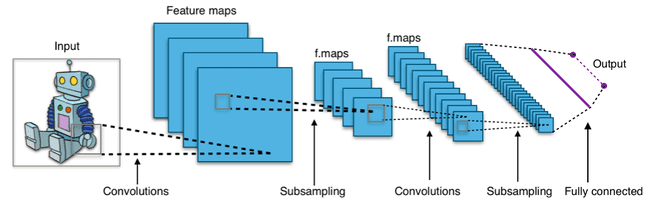
\includegraphics[width=0.5\textwidth, height=0.15\textheight]{convolution_diagram.png}
    \caption{\cite{Moor2017}}
    \label{fig:convolution_diagram}
\end{figure}

Het werkt als volgt: 

De eerste laag is meestal een convolutionele laag, die een reeks filters toepast op de invoergegevens. Elke filter is een kleine matrix van gewichten die over de ingevoerde gegevens schuift en op elke positie een puntproduct berekent. Het resultaat is een set feature maps die verschillende patronen in de invoergegevens benadrukken.

De volgende laag is meestal een poollaag, die de grootte van de feature maps verkleint door de maximale of gemiddelde waarde in elke lokale regio te nemen. Dit helpt om het aantal parameters in het model te verminderen en het efficiënter te maken.

Na verschillende convolutionele en pooling-lagen wordt de uitvoer afgevlakt en door een of meer volledig verbonden lagen geleid, die classificatie- of regressietaken uitvoeren op basis van de geëxtraheerde kenmerken.

Naast deze basislagen zijn er ook andere soorten lagen die kunnen worden gebruikt, zoals uitvallagen om overfitting te voorkomen, batch-normalisatielagen om de trainingsstabiliteit te verbeteren en activeringslagen om niet-lineariteit in het model te introduceren.

\cite{li2021survey}

\subsection{Recurrente neurale netwerken}

Een recurrent neuraal netwerk (RNN) is heel wat complexer dan een convolutioneel neuraal netwerk (CNN). 

Een RNN onthoud de output van een node en voedt het resultaat terug aan het model, via deze manier kan het niet enkel rekening houden met de huidige input, maar ook met alle andere voorgaande inputs. Onder andere hierin verschillen ze van een CNN, dat informatie maar in één richting doorgeeft.

\begin{figure}[htbp]
    \centering
    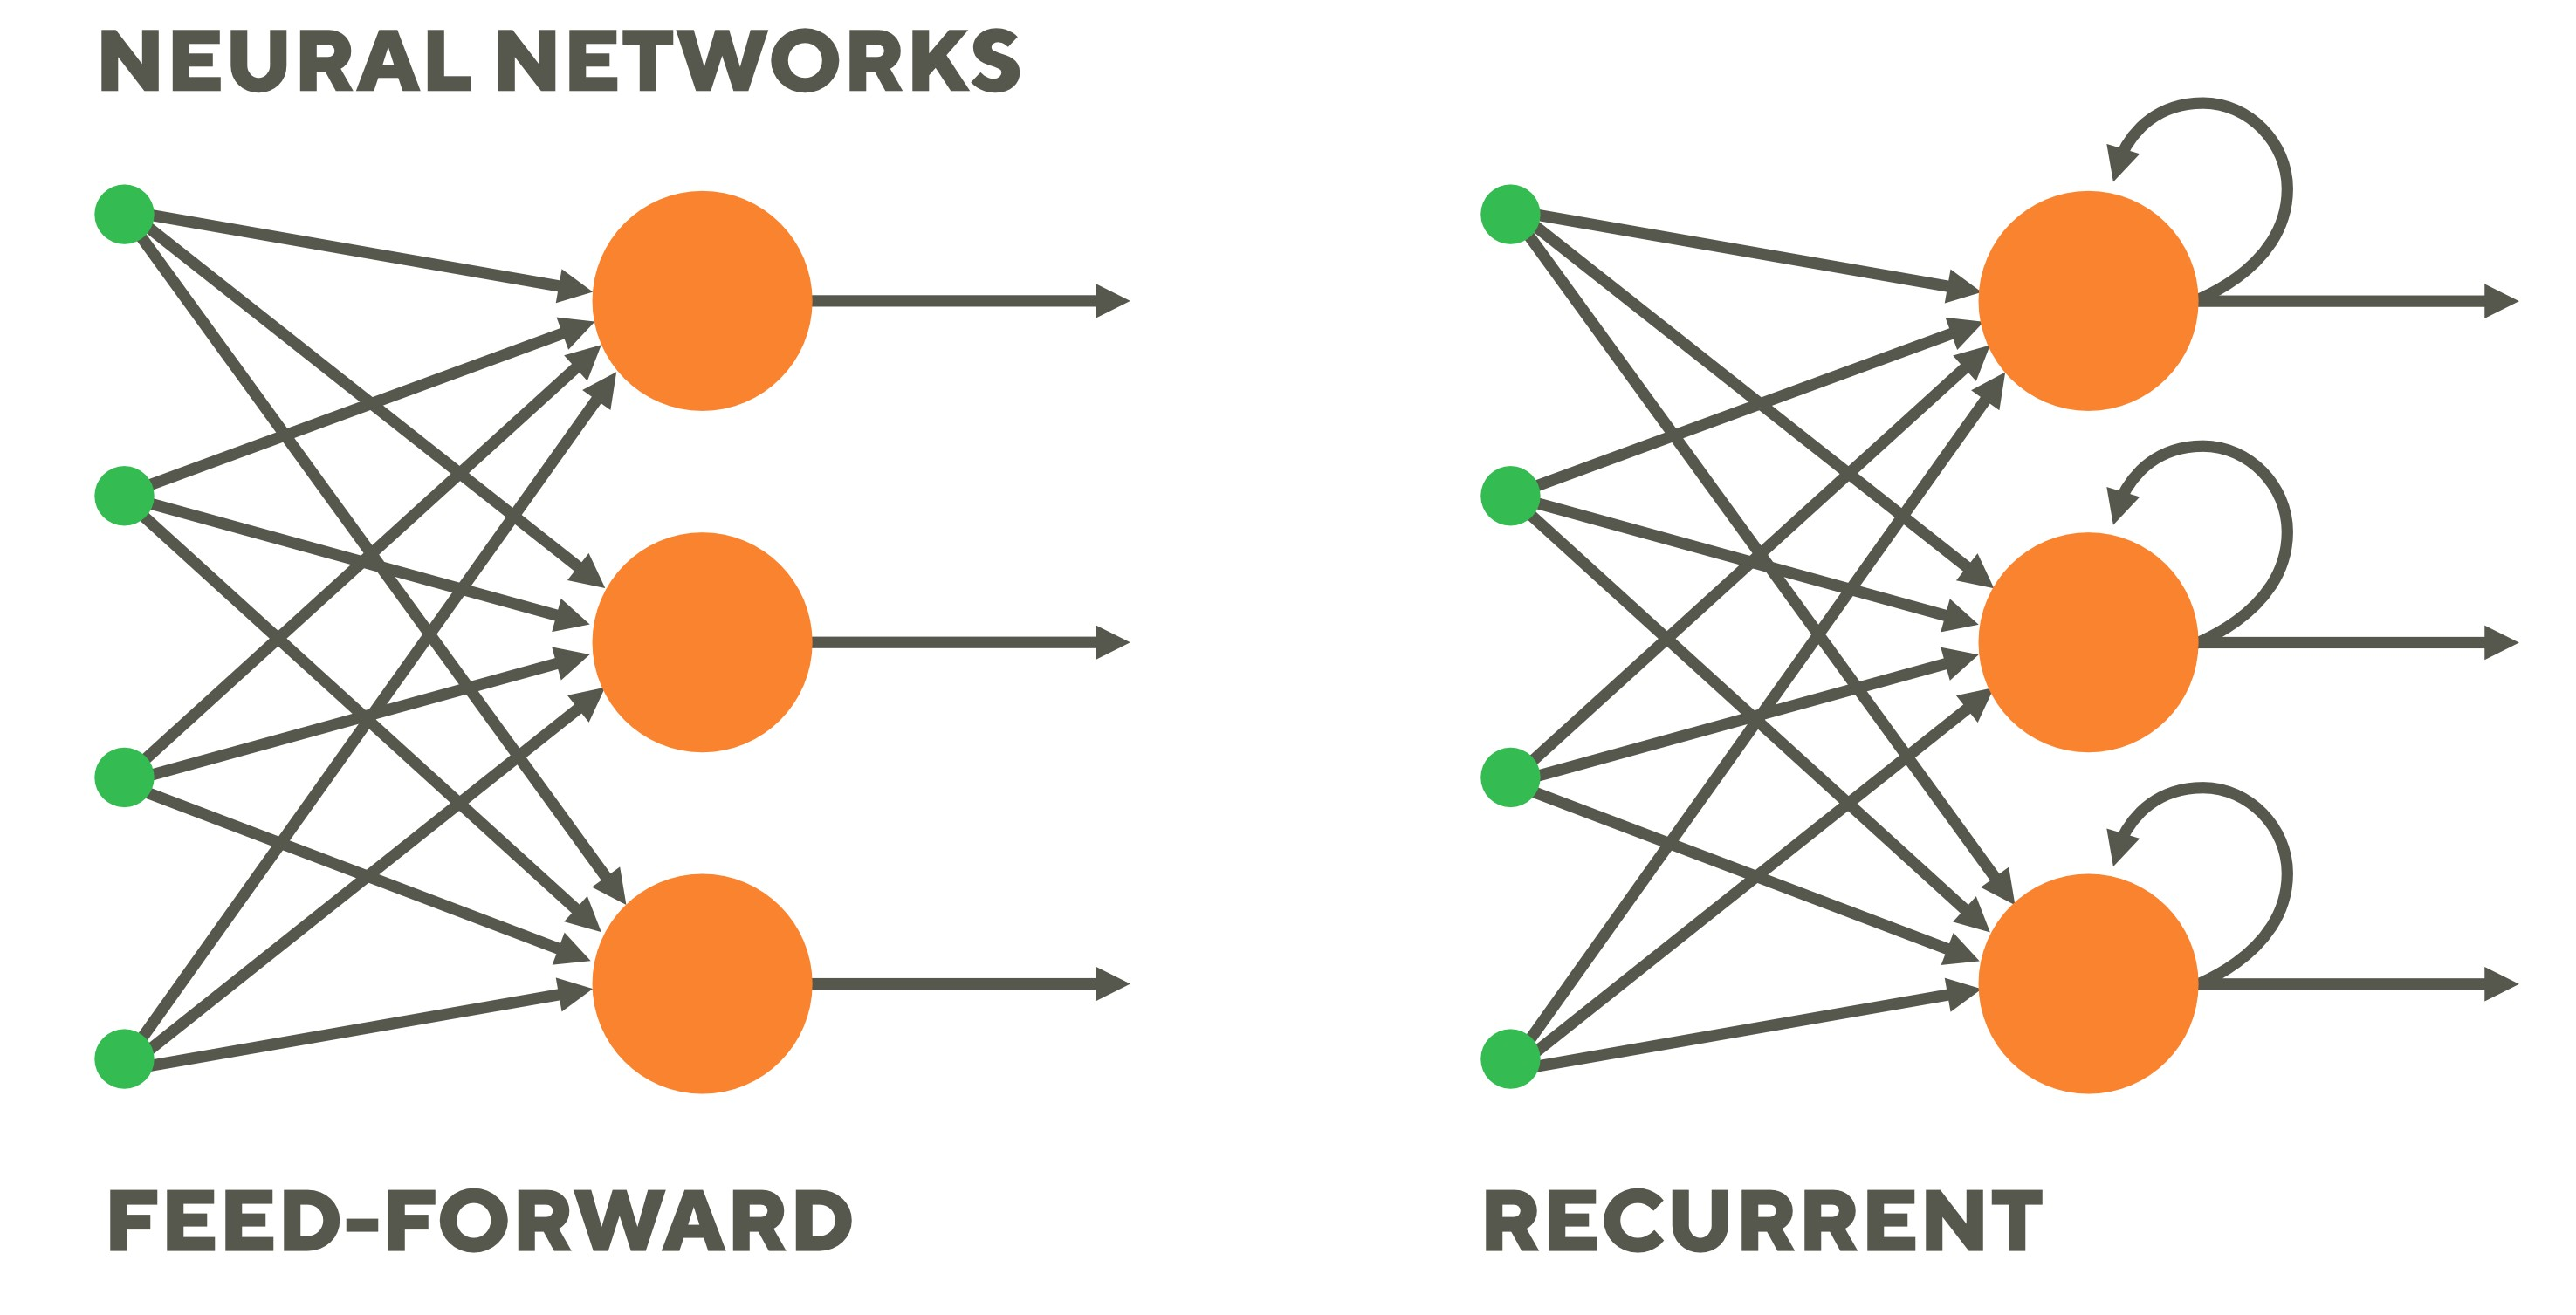
\includegraphics[width=0.5\textwidth]{OCS_NLP_RNN.jpg}
    \caption{\cite{Kerdijk2020}}
    \label{fig:recurrent_diagram}
\end{figure}

Een RNN wordt meestal gebruikt als men patterns wil herkennen in een sequentie van data, bij een CNN is dit voornamelijk afbeeldingsdata.

Een RNN komt vaak voor binnen taalmodelering, tekstgeneratie en spraakherkenning.

\cite{schmidt2019recurrent}

\subsection{Machine learning}

Machine learning is een vakgebied dat zich richt op het ontwikkelen van algoritmen en statistische modellen waarmee computersystemen kunnen leren aan de hand van data en voorspellingen kunnen doen of beslissingen kunnen nemen op basis van diezelfde data, zonder expliciet geprogrammeerd te zijn. 

Het omvat het trainen van een computersysteem om patronen in gegevens te herkennen en die patronen vervolgens te gebruiken om voorspellingen te doen of beslissingen te nemen over nieuwe gegevens. Machine learning wordt gebruikt in een breed scala aan toepassingen, waaronder beeld- en spraakherkenning en natuurlijke taalverwerking.

\cite{biamonte2017quantum}

\subsection{Deep learning}

Deep learning is een subset van machine learning waarbij artificiele neurale netwerken worden getraind om patronen in gegevens te herkennen. Het wordt "diep" genoemd omdat het gaat om trainingsnetwerken met veel lagen, waardoor ze steeds complexere kenmerken uit input kunnen leren. Zo zijn CNN's en RNN's een voorbeeld van een manier van deep learning.

De motivatie voor het gebruik van deeplearning in bijvoorbeeld computervisie of natuurlijke taalverwerking is dat het de creatie van complexere modellen mogelijk maakt die patronen in grote datasets kunnen leren en herkennen. Diepgaande leermodellen kunnen automatisch kenmerken leren van ongelabelde gegevens, wat kan leiden tot betere prestaties bij taken zoals beeldclassificatie en taalvertaling. Ook kunnen deep learning-modellen worden getraind op grote hoeveelheden gegevens, wat kan helpen om hun nauwkeurigheid en generalisatiemogelijkheden te verbeteren.

\cite{yan2015deep}

\subsection{Generatief antagonistennetwerk (deepfakes)}

Deepfakes zijn een soort synthetische media die deep learning-algoritmen gebruiken om nepvideo's, afbeeldingen of audio-opnamen te maken die echt lijken. Ze omvatten het verwisselen van het gezicht van de ene persoon naar een andere persoon in een video of afbeelding, waardoor het lijkt alsof de persoon iets zegt of doet wat hij eigenlijk nooit heeft gedaan. 

\cite{mahmud2021deep}

Hier onder in figuur \ref{fig:deepfake_example} ziet u enkele voorbeelden van een paar deepfakes.

\begin{figure}[htbp]
    \centering
    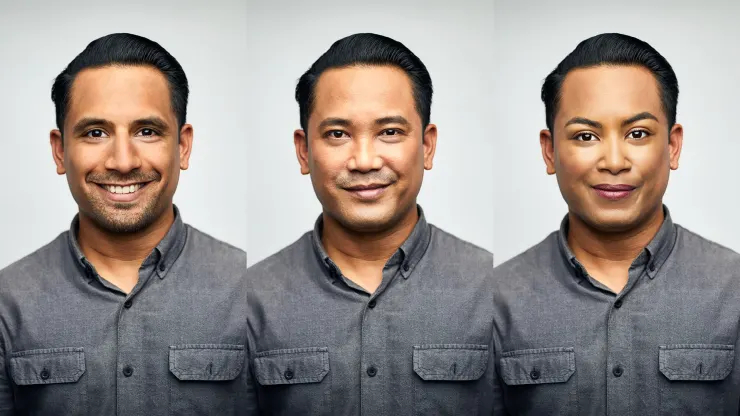
\includegraphics[width=0.5\textwidth, height=0.2\textheight]{deepfake.jpg}
    \caption{\cite{Walsh2021}}
    \label{fig:deepfake_example}
\end{figure}

Een generatief antagonistennetwerk is een soort neuraal netwerk dat uit twee delen bestaat: een generator en een discriminator. De generator creëert nieuwe items, zoals afbeeldingen, terwijl de discriminator ze evalueert op authenticiteit. De twee delen worden samen getraind in een proces dat vijandige training wordt genoemd, waarbij de generator probeert meer realistische gegevens te creëren om de discriminator te misleiden, de discriminator probeert vervolgens correct te identificeren of de gegevens echt of nep zijn. GAN's worden gebruikt voor verschillende toepassingen, waaronder het genereren van afbeeldingen en video's.

\cite{laino2022generative}

Deepfakes maken ook gebruik van GAN's. Zo kunnen ze hun uitkomst als maar beter maken door zich te trainen op misleiding, en zo als maar meer realistische fakes te genereren.

\subsection{Natuurlijke taalverwerking}

Natuurlijke taalverwerking is een onderzoeks- en toepassingsgebied dat onderzoekt hoe computers kunnen worden gebruikt om natuurlijke taal, tekst of spraak te begrijpen en te manipuleren om nuttige dingen te doen. Natuurlijke taalverwerking-onderzoekers streven ernaar kennis te verzamelen over hoe mensen taal begrijpen en gebruiken, zodat geschikte hulpmiddelen en technieken kunnen worden ontwikkeld om computersystemen natuurlijke talen te laten begrijpen en gebruiken om op deze manier gewenste taken uit te voeren.

Natuurlijke taalverwerking gebruikt verschillende technieken en tools om natuurlijke taal, tekst of spraak te analyseren en te begrijpen. Dit omvat morfologische analyses, lexicale en syntactische verwerking en het ontleden van zinnen. Natuurlijke taalverwerking systemen kunnen ook statistische en taalkundige criteria gebruiken om tekstdelen, zoals zinnen of paragrafen, te selecteren om samenvattingen te maken. 

Het uiteindelijke doel van NLP is om computers in staat te stellen natuurlijke taal te begrijpen en te gebruiken op een manier die vergelijkbaar is met hoe mensen dat doen.

\cite{chowdhary2020natural}

\subsection{Reinforcement learning}

Reinforcement learning is een vorm van machine learning waarbij een artificial intelligence leert om beslissingen te nemen, of taken uitvoert. De AI ontvangt feedback in de vorm van beloningen of sancties voor elke actie die hij onderneemt, en het doel is om te leren acties te ondernemen die de cumulatieve beloning in de loop van de tijd maximaliseren. 

Deze aanpak is geïnspireerd door de gedragspsychologie en kan worden toegepast op een breed scala aan opeenvolgende besluitvormingsproblemen in verschillende domeinen. Via deze manier kan men een AI trainen om telkens de betere keuze of beslissing uit te voeren.

\cite{franccois2018introduction}

\newpage

\subsection{Computer vision}

\begin{figure}[htbp]
    \centering
    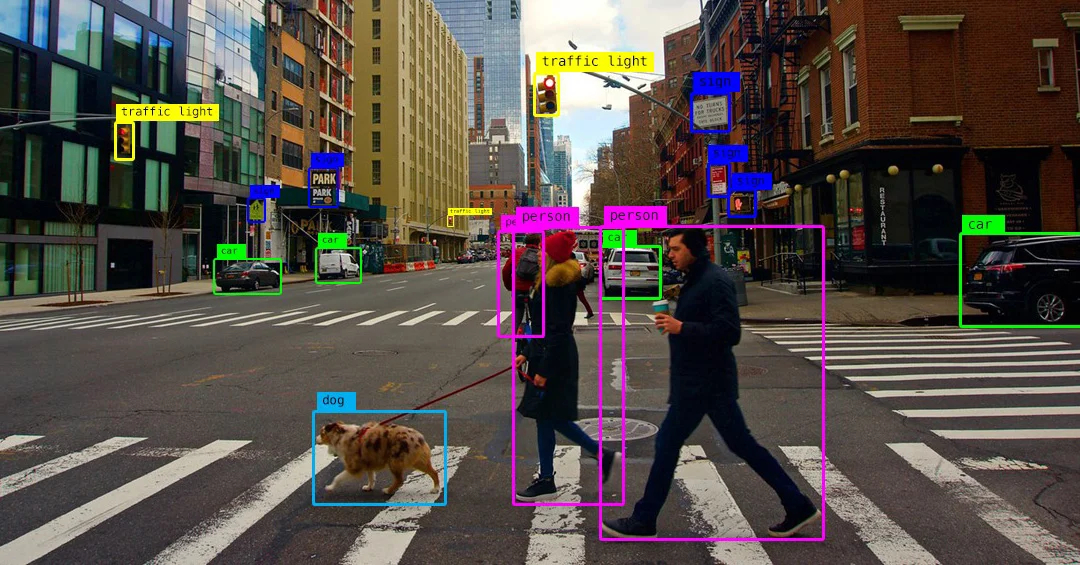
\includegraphics[width=1\textwidth]{Computervision_banner.jpg}
    \caption{\cite{Algotive2022computervision}}
    \label{fig:computervision_banner}
\end{figure}

Computer vision is een vakgebied dat zich richt op het in staat stellen van computers om visuele informatie uit de wereld om hen heen, zoals afbeeldingen en video's, te interpreteren en te begrijpen. Het omvat het ontwikkelen van algoritmen en technieken waarmee computers zinvolle informatie uit visuele gegevens kunnen analyseren, verwerken en extraheren, en die informatie kunnen gebruiken om beslissingen te nemen of acties te ondernemen.

Het proces omvat het gebruik van deep learning-methoden, zoals Convolutional Neural Networks (CNN's) om te leren uit data met meerdere abstractieniveaus, waarbij wordt nagebootst hoe de hersenen dit waarnemen. Deze deep learning modellen worden getraind op grote (openbaar beschikbare) gelabelde datasets van hoge kwaliteit. Eenmaal getraind, kunnen deze modellen worden gebruikt voor verschillende computervisietaken, zoals bijvoorbeeld objectdetectie en gezichtsherkenning.

\begin{figure}[htbp]
    \centering
    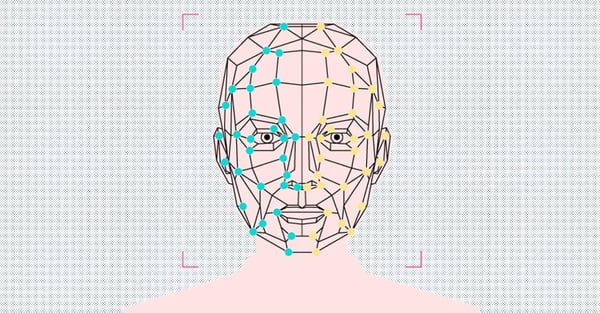
\includegraphics[width=0.5\textwidth]{face_recognition.jpg}
    \caption{\cite{AlgotiveAI2022}}
    \label{fig:computervision_facial}
\end{figure}

Computervisie omvat het gebruik van deze deep learning-modellen om visuele gegevens te analyseren en te interpreteren, waardoor computers de wereld om hen heen op een meer menselijke manier kunnen begrijpen en ermee kunnen omgaan.

\cite{voulodimos2018deep}

\subsection{Expert systemen}

Expertsystemen zijn computerprogramma's die artificiele intelligentie gebruiken om problemen in een specifiek domein op te lossen. Ze zijn ontworpen om het besluitvormingsvermogen van een menselijke expert binnen een bepaald gebied na te bootsen door kennis en een reeks regels te gebruiken om over informatie te redeneren en advies of aanbevelingen te geven. 

Expertsystemen worden gekenmerkt door hun vermogen om te redeneren met symbolische en wiskundige kennis, heuristische en algoritmische methoden te gebruiken, even goed te presteren als specialisten in hun probleemgebied, hun redenering begrijpelijk te maken en de nodige flexibiliteit te behouden.

\cite{buchanan1988fundamentals}

\subsection{Recommendatie systemen}

Recommendatie systemen zijn informatiefiltersystemen die helpen relevante en gepersonaliseerde inhoud of data uit een grote hoeveelheid data te vinden. Ze gebruiken algoritmen om gebruikersgegevens te analyseren, zoals gedrag in het verleden en voorkeuren. Dit kan ook gebruikt worden om aanbevelingen te doen voor nieuwe antwoorden of gespreksonderwerpen waarin de gebruiker mogelijks geïnteresseerd is.

\cite{isinkaye2015recommendation}

\subsection{Knowledge Graphs}

Knowledge graphs zijn een soort op graph gebaseerd gegevensmodel dat wordt gebruikt om kennis weer te geven in een gestructureerd en leesbaar formaat voor machines. Ze bestaan uit nodes die entiteiten vertegenwoordigen en edges die relaties tussen die entiteiten vertegenwoordigen. 

Kennisgrafieken worden gebruikt om kennis van de echte wereld te verzamelen en over te brengen, en kunnen worden opgevraagd en gevalideerd met behulp van verschillende grafische querytalen. Ze kunnen worden gebruikt in een verscheidenheid aan toepassingen, zoals aanbevelingssystemen en natuurlijke taalverwerking.

\cite{hogan2021knowledge}

\subsection{Patroonherkenning}

Patroonherkenning is het proces van het identificeren en classificeren van patronen in gegevens. Het omvat de automatische identificatie van patronen in gegevens, zoals afbeeldingen, spraak of tekst, en de classificatie van deze patronen in vooraf gedefinieerde categorieën. 

Het doel van patroonherkenning is om algoritmen en technieken te ontwikkelen die kunnen leren van gegevens en op basis van die gegevens nauwkeurige voorspellingen of beslissingen kunnen maken. Het kan gebruikt worden voor toepassingen binnen gebieden als beeld- en spraakherkenning.

\cite{basu2010use}

\subsection{Digitale signaalverwerking}

Digital Signal Processing (DSP) is het gebruik van wiskundige algoritmen om signalen in het digitale domein te manipuleren (versterken en verzachten) en te analyseren. Het omvat de verwerking van signalen zoals audio, video en afbeeldingen die zijn omgezet in een digitale vorm.

\cite{vaseghi2008advanced}

\subsection{Spraakherkenning}

Spraakherkenning is een technologie waarmee een computer menselijke spraak kan begrijpen en omzetten in tekst. Spraakherkenning gebruikt taalmodellen en akoestische modellen om gesproken woorden te identificeren en om te zetten in tekst. Er zijn echter nog steeds uitdagingen om de nauwkeurigheid van spraakherkenning te verbeteren, vooral met betrekking tot spraakvariabiliteit, zoals accenten, dialecten, spreeksnelheid, emoties, enz.

\cite{benzeghiba2007automatic}

\subsection{Text-to-speech}

Tekst to speech (TTS) is een technologie die geschreven tekst kan omzetten in gesproken woorden. Het is een proces van het synthetiseren van mensachtige spraak uit geschreven tekst met behulp van computeralgoritmen.

\cite{ren2019fastspeech}

